
%What is an auto encoder
\subsection{Autoencoder}
An autoencoder \cite{hinton2006reducing} is a type of artificial neural network designed to learn efficient representations of data, typically for the purpose of dimensionality reduction or feature learning through unsupervised learning. An autoencoder consists of two main components: an encoder and a decoder.

The encoder part of the network compresses the input 
$\mathbf{x} \in \R^n$ into a latent-space representation $\mathbf{z} \in \R^m$. Where $m < n$.

The encoder is defined by a function $\phi$:
\begin{equation}
    \mathbf{z}=\phi(\mathbf{x}).
    \label{eq:encoder}
\end{equation}
The output of the encoder, $\mathbf z$, is known as the latent space representation or the code. This compressed representation is intended to capture the most important features of the input data, facilitating tasks such as denoising, anomaly detection, and data compression.

The decoder reconstructs the input data from the latent representation. Similar to the encoder, the decoder consists of one or more layers and is typically a mirror image of the encoder architecture. It is defined by another function $\psi$:
\begin{equation}
\hat{\mathbf{x}}=\psi(\mathbf{z}).
\label{eq:decoder}
\end{equation}
The objective of an autoencoder is to minimize the reconstruction error, which measures the difference between the input $\mathbf{x}$ and the reconstructed output $\hat{\mathbf{x}}$. This is often done using a loss function $L$, such as the mean squared error:
\begin{equation}
L(\mathbf{x}, \hat{\mathbf{x}})=\|\mathbf{x}-\hat{\mathbf{x}}\|^2.     
\end{equation}
The overall optimization problem is to find the weights and biases of both the encoder and decoder network that minimize this loss

%Hva er Sindy
\subsection{SINDy}

\begin{figure}[H]
    \centering
    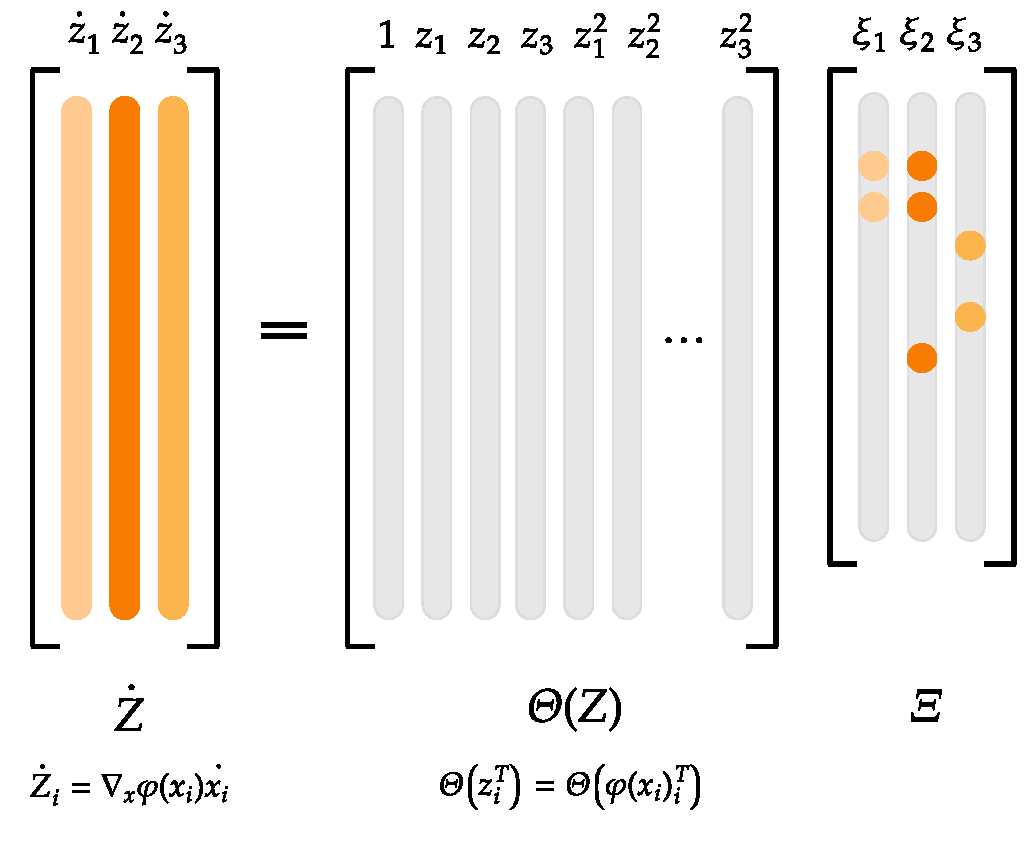
\includegraphics[width=0.48\textwidth]{project_2/images/SINDy_diagram.pdf}
    \caption{\textbf{SINDy diagram:} This figure shows a diagram of the true SINDy representation of the Lorenz system dynamics.}
    \label{fig:SINDy_diagram}
\end{figure}

The SINDy (Sparse Identification of Nonlinear Dynamics) algorithm is a procedure first described in the paper \cite{Brunton_2016} for taking time-series data and extracting interpretable and generalizable ODEs that describe the data. If we use the SINDy algorithm to fit a first order ODE to our data, we aim to find the function $\mathbf{f}$ which best describes the relation:
\begin{equation}
\frac{d \mathbf{x}}{d t}=\mathbf{f}(\mathbf{x}),
\label{eq:ode}
\end{equation}
where $\mathbf{x} \in \mathbb{R}^n$ is the state vector.% and $\mathbf{f}(\mathbf{x})$ represents the unknown nonlinear functions governing the system dynamics. Then the goal of SINDy is to identify $\mathbf{f}(\mathbf{x})$ from measurements of $\mathbf{x}$.

Given time-series data $\left\{\mathbf{x}\left(t_1\right), \mathbf{x}\left(t_2\right), \ldots, \mathbf{x}\left(t_m\right)\right\}$ and corresponding derivatives with respect to time $\left\{\dot{\mathbf{x}}\left(t_1\right), \dot{\mathbf{x}}\left(t_2\right), \ldots, \dot{\mathbf{x}}\left(t_m\right)\right\}$ We can construct a library $\Theta(\mathbf{x})$ containing $p$ candidate functions that might describe the dynamics:
\begin{equation}
\Theta(\mathbf{x})=\left[\begin{array}{llll}
\theta_1(\mathbf{x}) & \theta_2(\mathbf{x}) & \cdots & \theta_p(\mathbf{x})
\end{array}\right].
\label{eq:sindy_library}
\end{equation}
Typical choices for $\Theta(\mathbf{x})$ include polynomials, trigonometric functions, and other nonlinear functions of the state variables. 

SINDy attempts to express these time derivatives $\dot{\mathbf{x}}$ as a linear combination of the candidate functions:
\begin{equation}
    \dot{\mathbf{x}}=\Theta(\mathbf{x}) \boldsymbol{\Xi},
    \label{eq:sindy_formulation}
\end{equation}
where $\boldsymbol{\Xi} \in \mathbb{R}^{p \times n}$. Consequently, SINDy aims to find $\boldsymbol{\Xi}$ by solving the sparse regression problem:
\begin{equation}
    \boldsymbol{\Xi}=\arg \min _{\boldsymbol{\Xi}}\|\dot{\mathbf{x}}-\Theta(\mathbf{x}) \boldsymbol{\Xi}\|_2+\lambda\|\boldsymbol{\Xi}\|_1,
    \label{eq:sindy_loss}
\end{equation}
where $\|\cdot\|_2$ is the $\mathrm{L} 2$ norm, $\|\cdot\|_1$ is the $\mathrm{L} 1$ norm promoting sparsity, and $\lambda$ is a regularization parameter. Sparsity is used to encourage parsimonious models. Once $\boldsymbol{\Xi}$ is determined, the non-zero entries in each column of $\boldsymbol{\Xi}$ correspond to the predicted active terms in the governing equations for each state variable:
\begin{equation}
\frac{d x_i}{d t}=\sum_{j=1}^p \xi_{ij} \theta_j(\mathbf{x}),    
\end{equation}
where $\xi_{ij}$ denotes the indices of $\Xi$.
%Hva er autoencoder SINDY
\subsection{Autoencoder SINDy}
A drawback of using the vanilla SINDy algorithm is that the data might be unnecessarily complex when represented in its original coordinates. 
A naive approach to solve this would be to apply an autoencoder to the data in isolation and then use SINDy on the possibly simpler latent space, i.e. solving for
\begin{equation}
    \dot{\mathbf{z}}=\Theta(\mathbf{z}) \boldsymbol{\Xi}.
\end{equation}
However, this does not ensure that the coordinates learned by the autoencoder will be suitable for finding sparse dynamical models. 

A further development to this issue is proposed by \textcite{Champion_2019}. 
They present a method for the simultaneous discovery of sparse ODEs and PDEs, along with the coordinates that enable these simple representations. 
The paper details how to integrate a SINDy model with an autoencoder network to perform joint optimization.
\autoref{fig:autoencoder_sindy} displays how SINDy is integrated into the autoencoder. 
\begin{figure}[H]
    \centering
    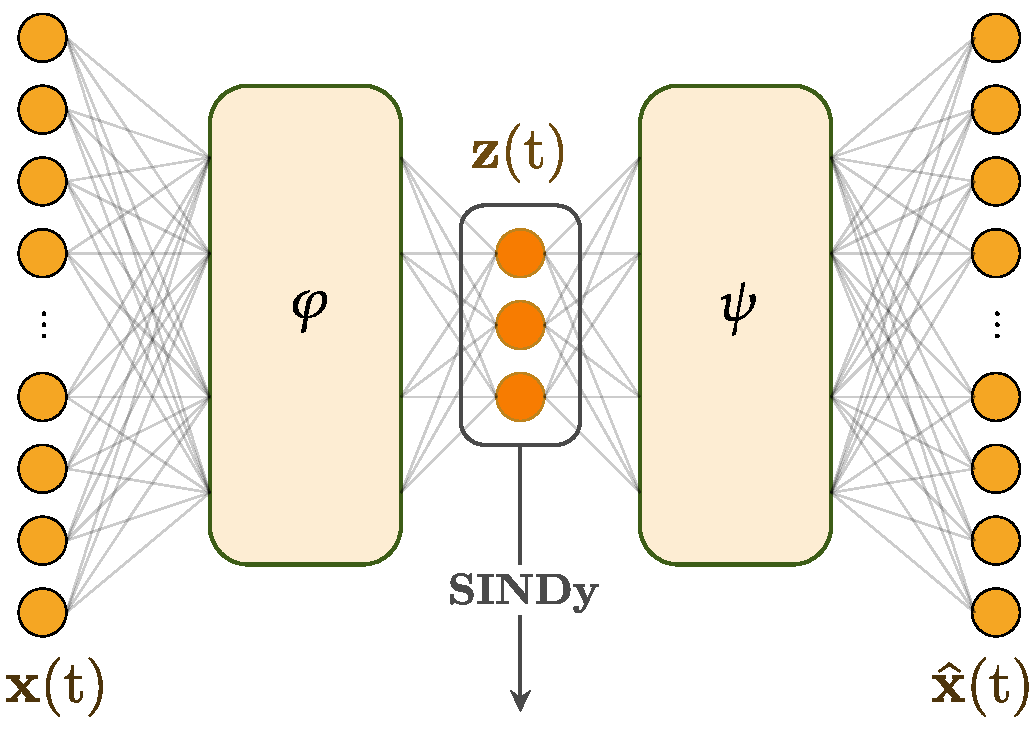
\includegraphics[width=0.48\textwidth]{project_2/images/autoencoder_diagram.pdf}
    \caption{\textbf{SINDy autoencoder diagram:} This figure shows a diagram of an autoencoder, where a SINDy model is applied in the latent space.}
    \label{fig:autoencoder_sindy}
\end{figure}
Joint-optimization of SINDy and the autoencoder is achieved by including terms in the loss function that enforce the accurate prediction of the dynamics in both the latent space and the original space. 
The library $\mathbf\Theta$ must still be decided beforehand, but the coefficients of $\mathbf\Xi$ are learned together with the autencoder parameters.

The loss functions can be understood by considering the derivatives of the encoder (\ref{eq:encoder}) and decoder (\ref{eq:decoder}) with respect to time. 

In the loss for fitting first order ODEs we require the first order derivatives.

\begin{equation}
     J_{\phi} (\mathbf{x})  \dot{\mathbf{x}} = \dot{\mathbf{z}}
\end{equation}

is what our SINDy part, $\boldsymbol{\Theta}(\mathbf{z}) \boldsymbol{\Xi}$, aims to predict. Thus giving us our loss in $\mathbf{z}$ space:
$$
\mathcal{L}_{\mathbf{z}}=\left\|J_{\phi}(\mathbf{x}) \dot{\mathbf{x}}-\boldsymbol{\Theta}(\mathbf{z}) \boldsymbol{\Xi}\right\|^2.
$$

The differentiating the decoder with respect to time gives:

\begin{equation}
\label{eq: dx_in_z}
    J_{\psi} (\mathbf{z}) \dot{\mathbf{z}}.
\end{equation}

This can be thought of as the derivative of $\hat{\mathbf{x}}$. Recalling that we want SINDy to predict $\dot{\mathbf{z}}$ leads to the formulation of our loss in \(\mathbf{x}\) space.
$$
\mathcal{L}_{\mathbf{x}} = \left\|\dot{\mathbf{x}} - \left(J_{\psi}(\mathbf{z})\right) \boldsymbol{\Theta}(\mathbf{z}) \boldsymbol{\Xi}\right\|^2
$$

For fitting second order ODEs we simply differentiate our encoder, $\phi$, and decoder, $\psi$, again and insert the same terms. 

Differentiating equation \ref{eq: dx_in_z} gives:

\begin{equation}
H_{\phi} (\mathbf{x}) \dot{\mathbf{x}} \dot{\mathbf{x}} + J_{\phi} (\mathbf{x}) \ddot{\mathbf{x}} = \ddot{\mathbf{z}},
\end{equation}.

This is what we wish our SINDy model to predict, $\ddot{\mathbf{z}}$. Since this is a second-order ODE, it may include $\mathbf{z}$ terms as well as $\dot{\mathbf{z}}$ terms. Therefore, it is reasonable to apply our library functions, $\boldsymbol{\Theta}$, to the state vector $\begin{bmatrix} \mathbf{z} & \dot{\mathbf{z}} \end{bmatrix}^T$. $\dot{\mathbf{z}}$ is calculated using equation~\ref{eq: dx_in_z}.

Combining this gives us our loss in $\mathbf{z}$ for second order ODEs:

\begin{equation}
\label{eq: loss_z_2}
    \mathcal{L}_{\mathbf{z}} = \left\|H_{\phi} (\mathbf{x}) \dot{\mathbf{x}} \dot{\mathbf{x}} + J_{\phi} (\mathbf{x}) \ddot{\mathbf{x}} - \boldsymbol{\Theta}\left(\begin{bmatrix} \mathbf{z} & \dot{\mathbf{z}} \end{bmatrix}^T\right) \boldsymbol{\Xi}\right\|^2.
\end{equation}

Differentiating our decoder again gives:

\begin{equation}
\label{eq: dx_in_z}
    H_{\psi} (\mathbf{z}) \dot{\mathbf{z}} \dot{\mathbf{z}} + J_{\psi} (\mathbf{z})\dot{\mathbf{z}} \ddot{\mathbf{z}}.
\end{equation}

This can be thought of as the double partial derivative with respect to time of $\hat{\mathbf{x}}$. Doing the the same substitutions, we did for equation \ref{eq: loss_z_2}, we recover the loss in $\mathbf{x}$:

\begin{equation}
    \mathcal{L}_{\mathbf{x}} = \left\| \ddot{\mathbf{x}} -     H_{\psi} (\mathbf{z}) \dot{\mathbf{z}} \dot{\mathbf{z}} + J_{\psi} (\mathbf{z})\dot{\mathbf{z}}\boldsymbol{\Theta}\left(\begin{bmatrix} \mathbf{z} & \dot{\mathbf{z}} \end{bmatrix}^T\right) \boldsymbol{\Xi}   \right\|.
\end{equation}




The overall loss function combines the reconstruction error, the SINDy model errors in both the latent space and the original space, and an L1 regularization term to promote sparsity of the coefficients:
\begin{equation}
    \mathcal{L}=\mathcal{L}_{\text {recon }}+\lambda_1 \mathcal{L}_{\mathbf{x}}+\lambda_2 \mathcal{L}_{\mathbf{z}}+\lambda_3\|\mathbf{\Xi}\|_1
\end{equation}
where $\lambda_1, \lambda_2$, and $\lambda_3$ are hyperparameters that determine the relative weighting of each term.

% Dette hadde sett mye bedre ut på én linje
% Men vi har to kolonner fordi vi leker fysikere

\begin{comment}
\begin{align}
    \underbrace{\|\mathbf{x}-\psi(\mathbf{z})\|_2^2}_{\text{reconstruction loss}}
    + \underbrace{\lambda_1\left\|\dot{\mathbf{x}}-\left(\nabla_{\mathbf{z}} \psi(\mathbf{z})\right)\left(\boldsymbol{\Theta}\left(\mathbf{z}^T\right) \boldsymbol{\Xi}\right)\right\|_2^2}_{\text{SINDy loss in } \dot{\mathbf{x}}} \notag 
    \\
     + \underbrace{\lambda_2\left\|\left(\nabla_{\mathbf{x}} \mathbf{z}\right) \dot{\mathbf{x}}-\boldsymbol{\Theta}\left(\mathbf{z}^T\right) \boldsymbol{\Xi}\right\|_2^2}_{\text{SINDy loss in } \dot{\mathbf{z}}}
    + \underbrace{\lambda_3\|\boldsymbol{\Xi}\|_1}_{\text{SINDy regularization}}
\end{align}

\end{comment}

%To ensure a parsimonious model, \textcite{Champion_2019} employs the sequential thresholding least-squares algorithm during training, setting coefficients below a certain threshold to zero at fixed intervals, promoting sparsity in the same way as $L_0$ regularization by penalizing solutions with an abundance of coefficients. 
To ensure a parsimonious model, \textcite{Champion_2019} employs sequential thresholding with gradient-based optimization during training. This process sequentially eliminates coefficients from $\boldsymbol{\Xi}$ that are below a certain threshold, which can sometimes be considered a fourth loss parameter, $\lambda_4$. In practice, this is performed using masking. This approach promotes sparsity by removing small coefficients, making the model more interpretable and potentially more generalizable.

%The technique described by Champion reduces the complexity of the problem which potentially lets the joint autoencoder SINDy algorithm uncover the underlying structure of the problem more easily than the plain SINDy algorithm.
%\subsection{Second order loss function}
%Note that the previous autoencoder SINDy loss formulation only applies to the case where one wishes to determine first-order derivatives. 
%For second-order equations, additional work is needed to determine the losses. 
%Hence, by applying the chain rule, one arrives at the following loss formulations:
%\begin{equation*}
%    \mathcal L_{\ddot{x}} = \|\ddot{x} - \|
%\end{equation*}


\subsection{Backpropagation}
Backpropagation consists of two main components: automatic differentiation and gradient-based optimization. During the forward pass, the network output and loss are computed. In the backward pass, automatic differentiation calculates the gradients of the loss with respect to each weight. These gradients are then used in gradient-based optimization methods to update the network's weights and biases, minimizing the loss function over successive iterations.

Consider a neural network with $L$ layers, where $l=1,2, \ldots, L$. Each layer $l$ has $n_l$ neurons. The input to the network is $\mathbf{x}$, and the output is $\hat{\mathbf{y}}$.

For each layer $l$ we can compute the weighted input $\mathbf{z}^{(l)}$ :
$$
\mathbf{z}^{(l)}=\mathbf{W}^{(l)} \mathbf{a}^{(l-1)}+\mathbf{b}^{(l)}
$$
where $\mathbf{W}^{(l)}$ is the weight matrix, $\mathbf{a}^{(l-1)}$ is the activation from the previous layer, and $\mathbf{b}^{(l)}$ is the bias vector. We can apply the activation function $g$ to obtain the next activation $\mathbf{a}^{(l)}$ :
$$
\mathbf{a}^{(l)}=g\left(\mathbf{z}^{(l)}\right)
$$
The model behaviour determined by these weights and biases is then evaluated in the loss function. Which measures how poorly our model performed.
%Then we can use this prediction to compute the loss function $\mathcal{L}(\hat{\mathbf{y}}, \mathbf{y})$ which quantifies the error between the predicted output $\hat{\mathbf{y}}$ and the true target output $\mathbf{y}$.

With the calculated loss we can use backpropogation to compute the gradient of the loss function with respect to each weight $\mathbf{W}^{(l)}$ and bias $\mathbf{b}^{(l)}$. 

The error $\delta^{(L)}$ at the output layer is given by:
$$
\delta^{(L)}=\nabla_{\mathbf{a}^{(L)}} \mathcal{L} \odot g^{\prime}\left(\mathbf{z}^{(L)}\right)
$$
where $\odot$ is the elementwise product, $\nabla_{\mathbf{a}^{(L)}} \mathcal{L}$ is the gradient of the loss function with respect to the activation $\mathbf{a}^{(L)}$, and $g^{\prime}$ is the derivative of the activation function. For each layer $l=L-1, L-2, \ldots, 1$, we propagate the error backwards:
$$
    \delta^{(l)}=\left(\mathbf{W}^{(l+1)}\right)^T \delta^{(l+1)} \odot g^{\prime}\left(\mathbf{z}^{(l)}\right)
$$
And compute the gradients of the loss function with respect to $\mathbf{W}^{(l)}$ and $\mathbf{b}^{(l)}$ :
$$
\begin{gathered}
\nabla_{\mathbf{W}^{(l)}} \mathcal{L}=\delta^{(l)}\left(\mathbf{a}^{(l-1)}\right)^T \\
\nabla_{\mathbf{b}^{(l)}} \mathcal{L}=\delta^{(l)}
\end{gathered}
$$
Then we update the weights and biases using the computed gradients:
$$
\begin{aligned}
\mathbf{W}^{(l)} & \leftarrow \mathbf{W}^{(l)}-\eta \nabla_{\mathbf{W}^{(l)}} \mathcal{L} \\
\mathbf{b}^{(l)} & \leftarrow \mathbf{b}^{(l)}-\eta \nabla_{\mathbf{b}^{(l)}} \mathcal{L}
\end{aligned}
$$
where $\eta$ is the learning rate.
